\documentclass[11pt,french,a4paper]{article}
\usepackage[utf8]{inputenc}
\usepackage[french]{babel}
\usepackage[T1]{fontenc}
\usepackage{fancyhdr}
\usepackage{fancybox}
\usepackage{lastpage}
\usepackage{graphicx}
\usepackage[left=2cm,right=2cm,top=2cm,bottom=2.5cm]{geometry}
\geometry{a4paper}
\setlength{\parindent}{0pt}
\usepackage{listings}
\usepackage{color}
\usepackage[table]{xcolor}
\usepackage{array}
\usepackage{listings}
\usepackage{hyperref}
\usepackage{caption}
\usepackage{lastpage}
\pagestyle{fancy}

\fancyhead[L]{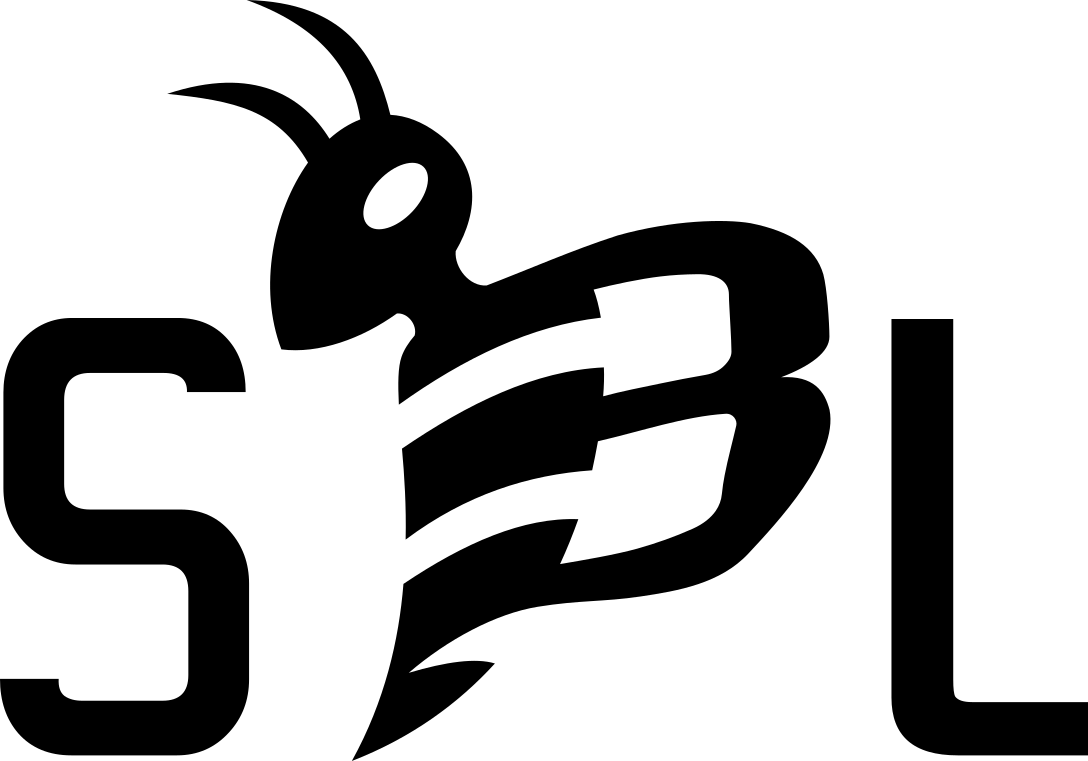
\includegraphics[width=1cm]{../../../logo/SBLlogo.png}}
\fancyhead[C]{Rapport d'activités semaines du 11 et 18 avril 2022 }
\fancyhead[R]{}
\fancyfoot[L]{\small Tom TUELEAU\normalsize}
\fancyfoot[C]{}
\fancyfoot[R]{\thepage/\pageref{LastPage}}


\lstset{
  basicstyle=\fontfamily{lmvtt}\selectfont\small,
  columns=fullflexible,
}

\title{
 \centering
         
\includegraphics[width=4cm]{../../../logo/IUTlogo.png}  \hspace{7cm}
         
\includegraphics[width=4cm]{../../../logo/UMlogo.png}  \hspace{7cm}
    
	\LARGE{Rapport d'activiter du 11 et 18 avril 2022}
	\author{TUELEAU Tom}
}
\author{
	\date{}
}
\begin{document}
\maketitle
	 
\includegraphics[width=4cm]{../../../logo/LIRMMlogo.png}  \hspace{7cm}
         \includegraphics[width=4cm]{../../../logo/IBMMlogo.jpg}  \hspace{7cm}
\newpage
\tableofcontents
\newpage
\section{Introduction}
Ce document a pour objectif de faire un état d'avancement du stage. Celui-ci résumera donc le travail effectué lors des semaines du 11 et 18 avril 2022.
\\Je vais vous présenter dans un premier temps les recherches que j'ai pu effectuer sur le Piezo-Electrique les AOP ou encore la fréquence qu'émettent les abeilles. 
\\Dans une deuxième partie, je parlerais de la découverte du logiciel spice ainsi que les simulations que j'ai pu effectuée lors de ces 2 semaines.
\\Une troisiéme partie reviendra sur les résultats obtenu pour le capteur de vibration. 
\\Enfin, une dernière partie introduira les outils que j'ai mis en place pour m'organiser tout au long du projet. 

\newpage
\section{Recherche}
Comme dis en introduction, j'ai été amené à me documenter afin d'accomplir plusieurs objectifs. Le premier objectif était d'étudier les solution à ma disposition afin d'amplifier mon signal. Mes recherches se sont donc portées sur les amplificateurs opérationels. Mon second objectif était de faire des recherches sur le fréquence émise par les abeilles afin de commander des capteurs de vibrations avec une plage de fréquence adéquate. 
\subsection{AOP}
Ma principale source d'information pour cette partie a été Mr Druon m'ayant fournis plusieurs documentations sur les montages à amplificateur opérationnel. 
Mes recherches ont principalement consisté à tester des montages et à verifier par le calcul si les valeurs récupérées étaient les bonnes.
Je suis donc passé directement à de l'experimentation en testant comme vu lors du précédent rapport différents montages basiques.
Nous verrons plus en détail lors de la partie "Capteur de vibration" la mise en pratique de ces montages.

\subsection{Fréquence et piezo-electrique}
Afin de pouvoir mesurer avec plus de précisions les vibrations émises par les abeilles, j'ai pris conseil auprès de monsieur Rousset qui m'a fourni differents articles sur le sujet.
Apres une lecture de ces documents, je suis arrivé à une estimation de la plage de fréquence de communication des abeilles dans la ruche à [200Hz-1000Hz]. Je me base sur cet echange avec Mr ROUSSET pour déduire cette plage de valeurs : \\ 
\\
\\
\fbox{
	\begin{minipage}{17cm} 
Les vibrations dans les matériaux qui sont probablement détectées par plusieurs organes/structures dans le corps de l’abeille. Par exemple l’organe subgénual (subgenual organ) localisé dans la patte est sensible aux vibrations entre 200 et 1000Hz.
	\end{minipage}

}
\\ \\ \\Etant donné le temps restant avent la dead-line, j'ai préféré me baser sur ce résultat pour la commande des piézo-électrique.

\newpage
\section{Simulation}
Afin de pouvoir simuler les montages qu'il me sera nécessaire d'effectuer, il m'a été conseillé d'étudier et de me former sur le logiciel spice.

\subsection{ngspice}
Étant sur une distribution linux, j'ai installé le logiciel "ngspice". Celui-ci est Open Source et est installable trés facilement sur n'importe quelle distribution basée sur Unix. L'objectif principal pour moi est de pouvoir simuler mes montages afin d'étudier leur comportement. 

\subsection{Apprentissage du logiciel}
Lors de cette semaine d'apprentissage de spice j'ai pu apprendre les choses suivantes :
\\
\\
- Simuler un circuit de base avec resistor, condensateur, bobine, générateur de tension, génerateur de courant\\
- Créer un signal continue, sinusoidale et impulsionel \\
- Afficher les résultats de ceci à l'aide de graphiques \\

\subsection{Etat actuel}
Malgrés le temps investis sur celui-ci, je ne maitrise pas encore parfaitement le logiciel et suis encore entrain de le prendre en main. Je compte cependant tenter, dans la semaine à venir, de simuler le montage que vous verrez dans la prochaine partie. 
\newpage
\section{Capteurs de vibration}
Le capteur piezo-electrique ne produisant pas une tension assez élevée pour que je l’utilise telquel, j’ai donc dû trouver un moyen de l’amplifier. Je vais donc vous présenter les montages que j’ai pu étudiés et les résultats obtenus.

\subsection{Montage}
\subsubsection{Rappel}

Comme vu dans le rapport de la première semaine, j’ai commencé par faire des montages basiques (Suiveur, Amplificateur non-inverseur) composés d’amplificateur operationnel (AOP). Ceux-ci m’avaient posé des problèmes dus aux modèles d’AOP que j’utilise (LM741) qui nécessitent une alimentation en parallèle.

\subsubsection{Amplificateur de mesure}

Lors de cette semaine je suis donc passé au montage amplificateur de mesure. Ce montage est très souvent utilisé afin d’amplifier le signal de sortie d’un capteur ayant une tension trop faible.
Il existe plusieurs montages amplificateur de mesures. Dans mon cas, j’ai commencé par un montage nécessitant 3 AOP. Nous pouvons voir ce montage figure \ref{3AOP}

\begin{center}	
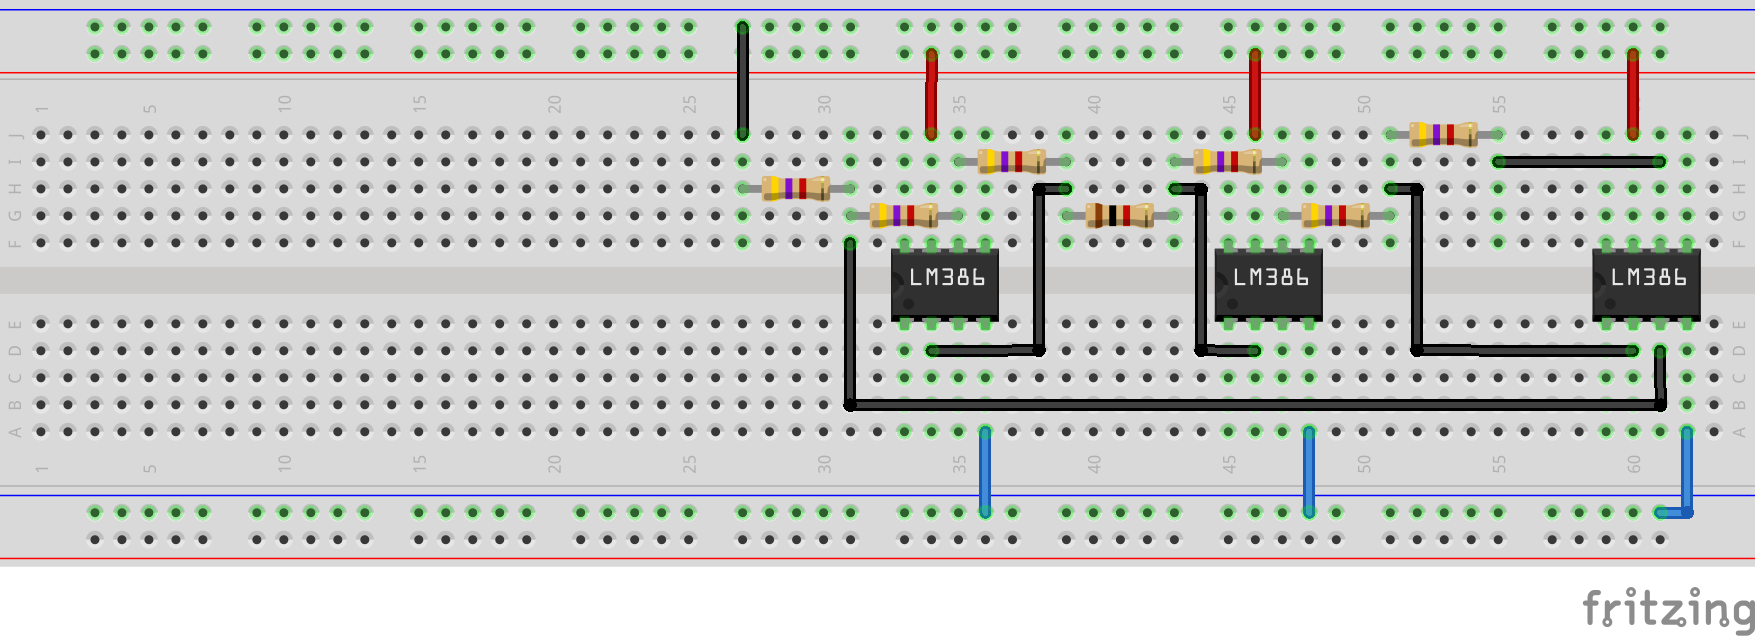
\includegraphics[scale=1]{../img/instrumentation3aop_bb.png}
\captionof{figure}{Montage 3 AOP sous Fritzing}
\label{3AOP}
\end{center}


Il existe cependant des montages plus simples notamment un, composé de deux amplificateurs opérationnels que l'on peut voir figure \ref{2AOP}.
\\

\begin{center}	
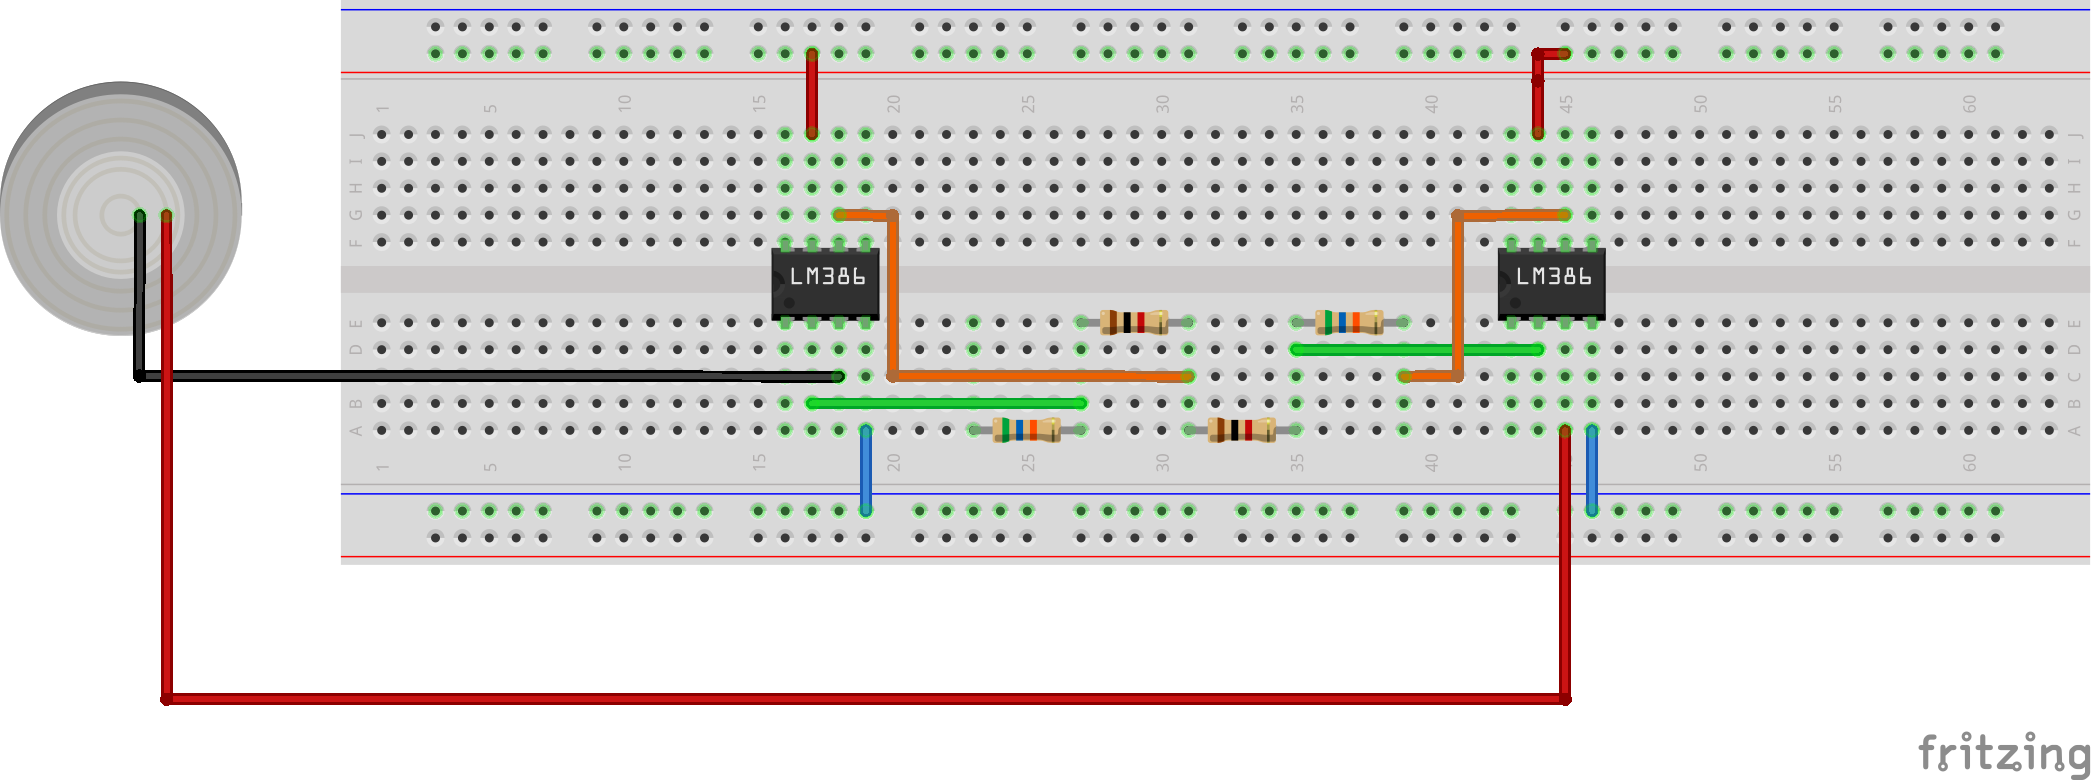
\includegraphics[scale=0.80]{../img/instrumentation2aop_bb.png}
\captionof{figure}{Montage 2 AOP sous Fritzing}
\label{2AOP}
\end{center}

Aprés avoir réussi à effectuer ce montage, j’ai pu remarquer que la sensibilité avait diminueé. Ceci a eu pour effet de d’empêcher la vision d’impulsion créée lors de petit frottement. Aprés plusieurs tentative de modification pour pallier à ce changement, j’ai décidé de changer de montage.

\subsubsection{Montage actuel}
Le piezo-electrique utilisé jusqu’a maintenant était fourni avec un module. Celui-ci ne changait rien au signal pour cause, les composants sur lui n’étaitent pas totalement connectés. Cependant, après avoir effectué des modifications sur celui-ci le signal m'a paru beaucoup plus net.
J’ai par la suite effecuté le montage visible figure \ref{MTGFINAL}
\\
\begin{center}	
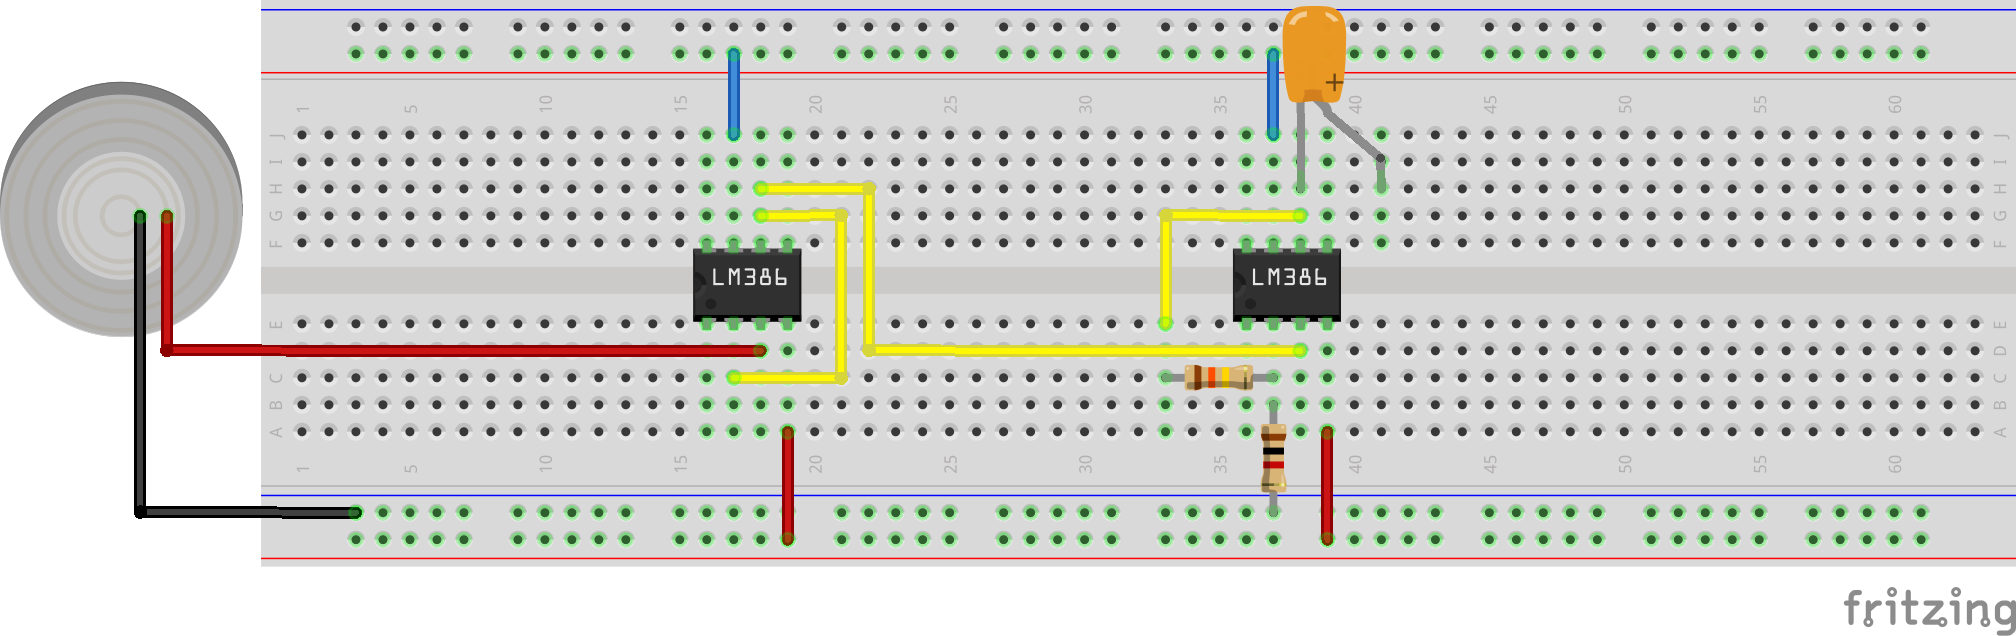
\includegraphics[scale=0.85]{../img/mtgfinal.png}
\captionof{figure}{Dernier montge }
\label{MTGFINAL}
\end{center}
Il est composé d’un amplificateur suiveur et d’un amplificateur non-inverseur avec un coefficient multiplicateur de 130. C'est à dire que la tension de sortie sera 130 fois la tension d'entrée. Enfin, un condensateur se trouvant en sortie de circuit nous permet d’éliminer la composante continue ajoutée par les AOP à notre signal.


\subsubsection{Résultat}
Avec le montage vue précédemment nous obtenons plusieurs résultats probants.
Tout d'abord, nous pouvons voir figure \ref{VWOMVM} le signal en sortie du montage quand aucun évenement ne se produit.
Ensuite figure \ref{F}, nous pouvons voir la réaction après un léger frottement effectué avec un câble visible figure \ref{M}. 

\begin{center}	
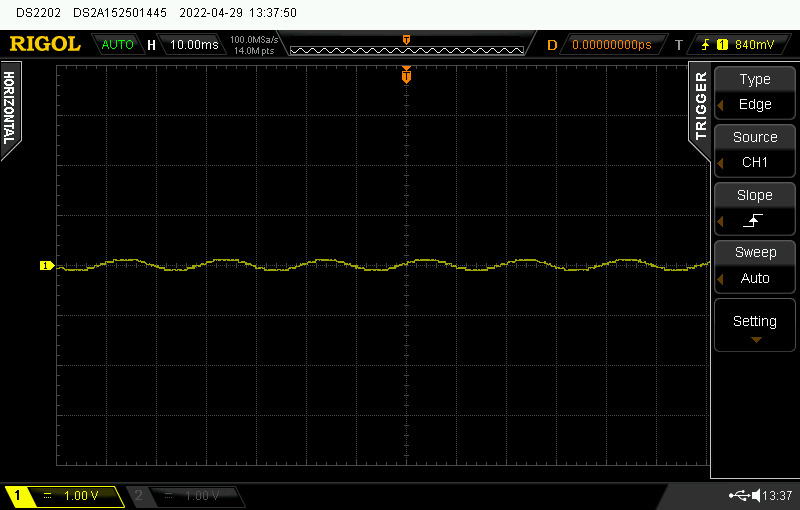
\includegraphics[scale=0.5]{../img/plat.jpg}
\captionof{figure}{Tension sans mouvement}
\label{VWOMVM}
\end{center}

\begin{center}	
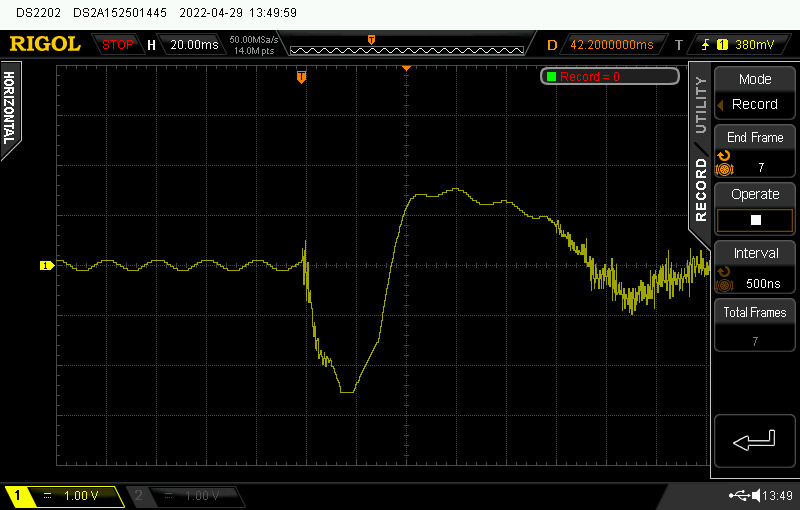
\includegraphics[scale=0.5]{../img/frotment.jpg}
\captionof{figure}{Tension lors d'un Frotement}
\label{F}
\end{center}

\begin{center}	
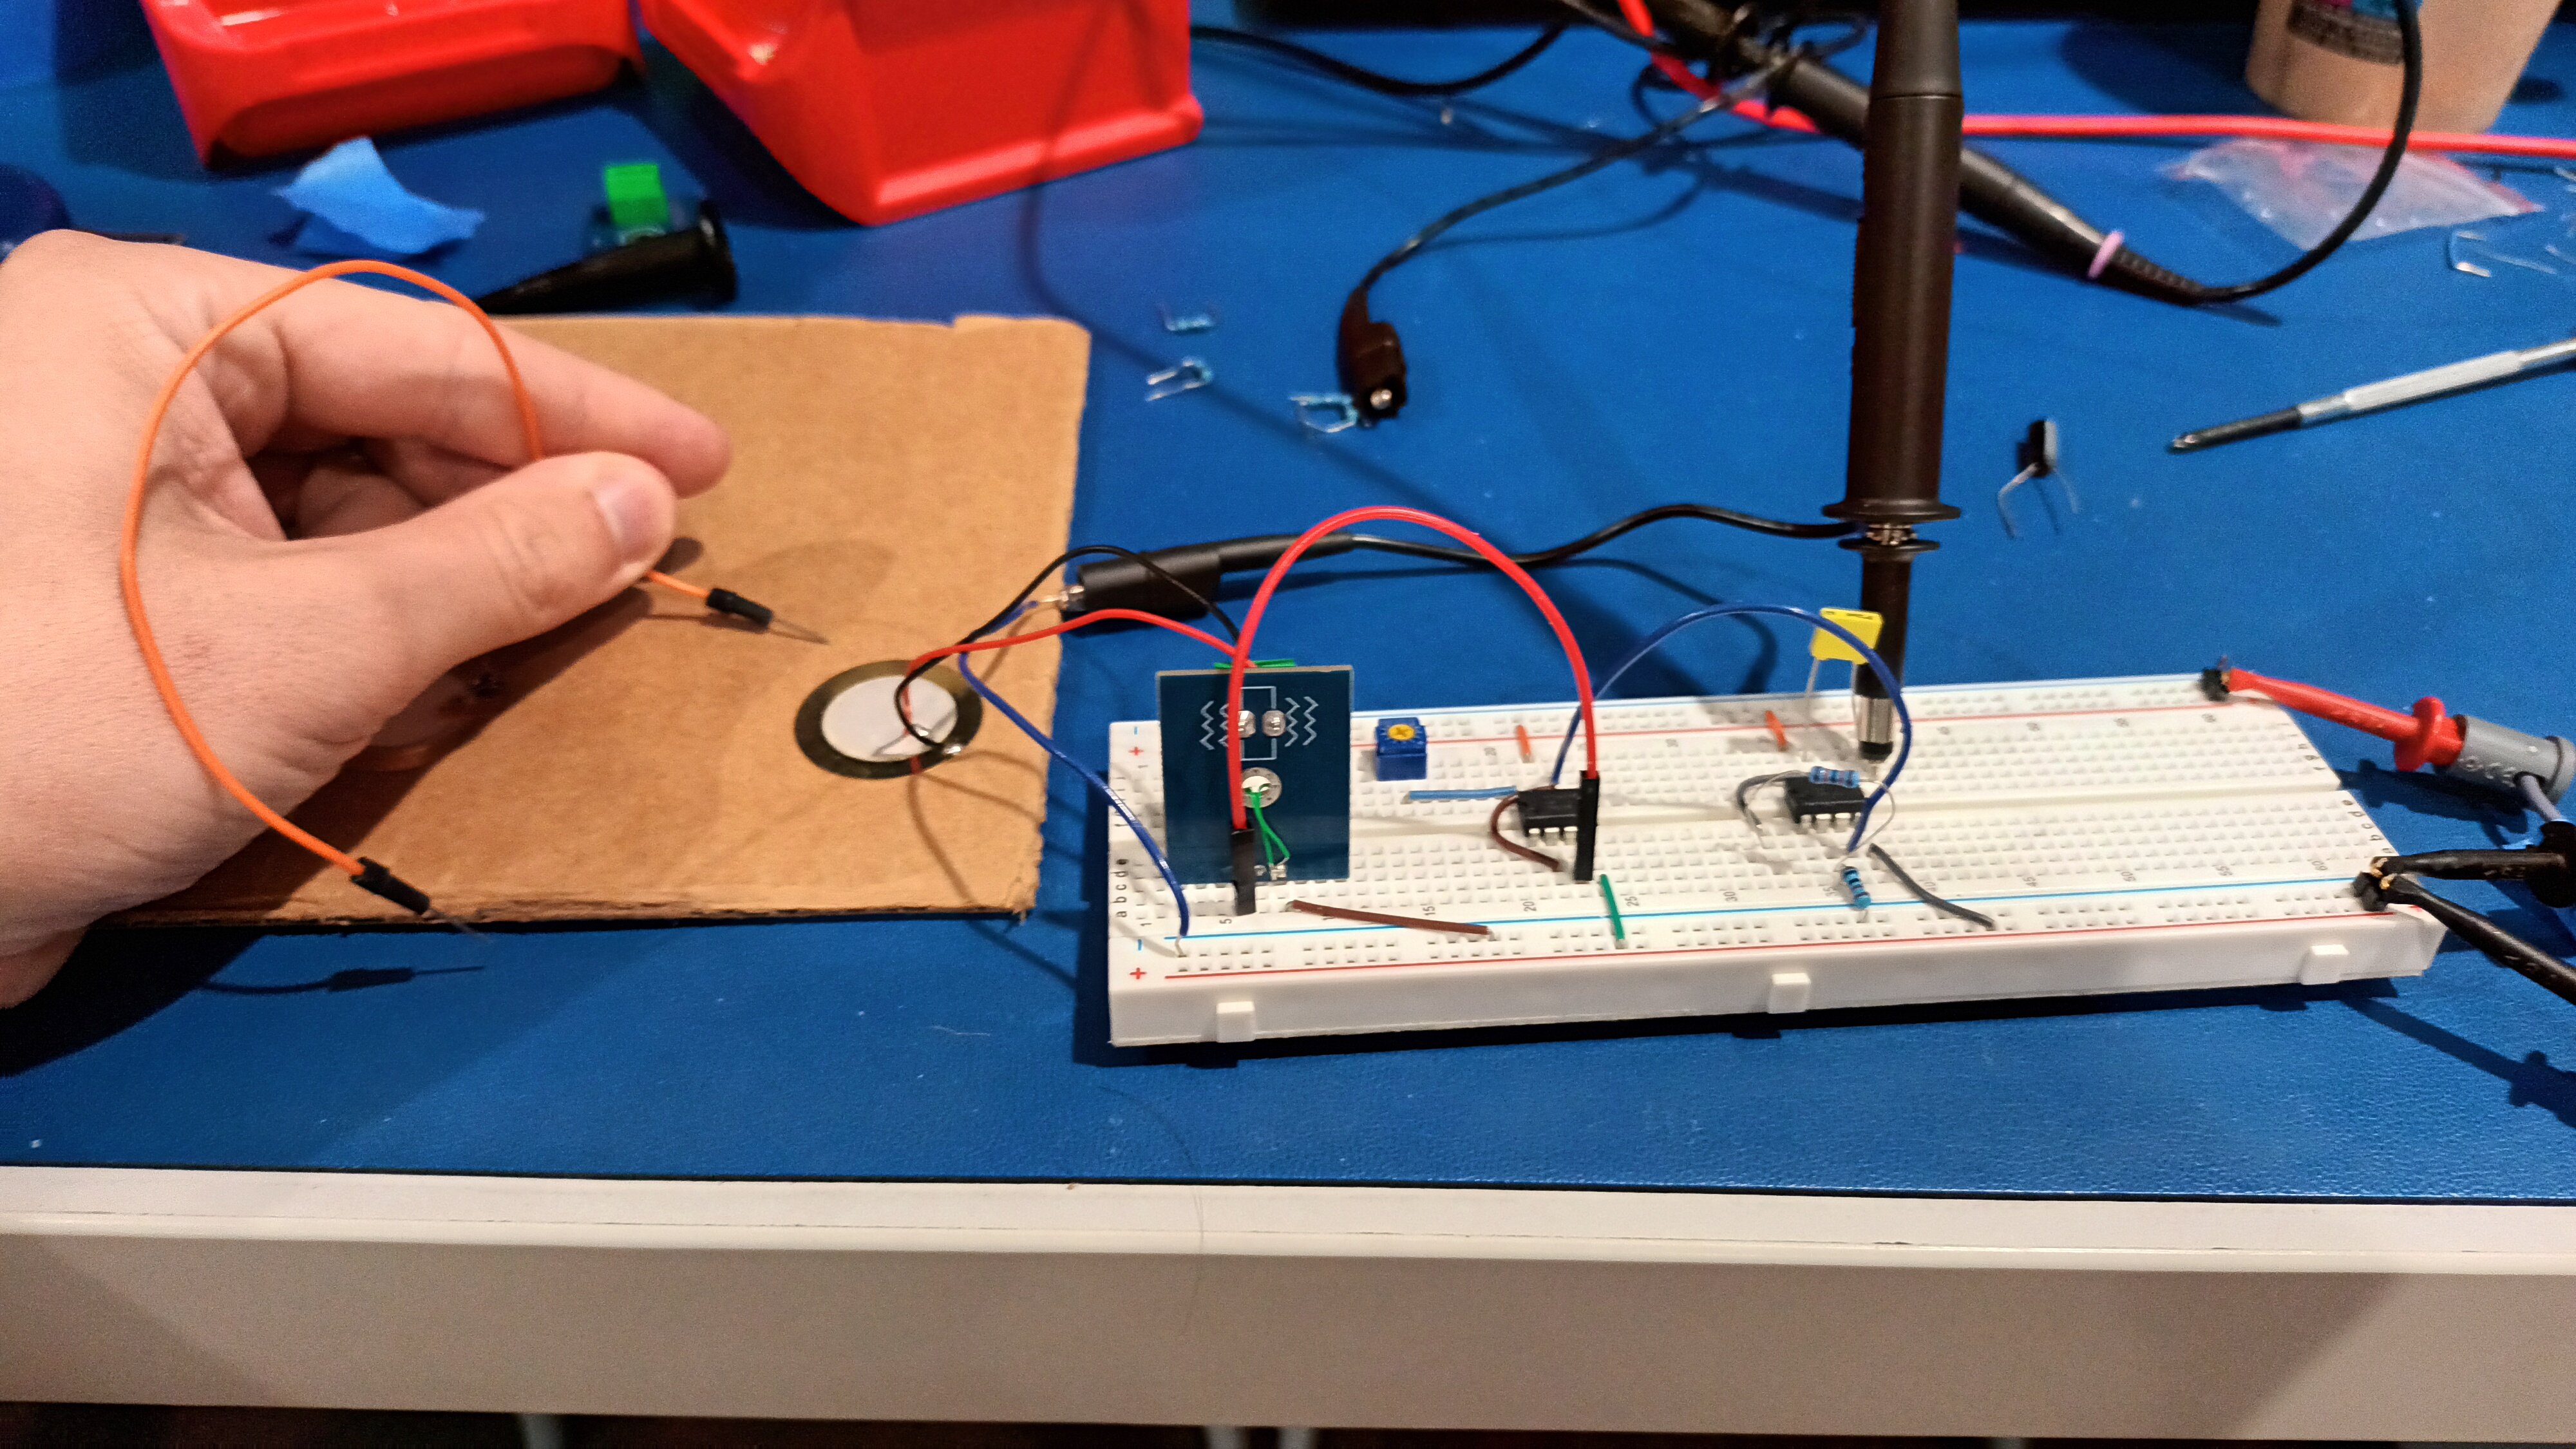
\includegraphics[scale=0.1]{../img/froty.jpg}
\captionof{figure}{Frotement}
\label{M}
\end{center}

\subsubsection{Conclusion}
Nous sommes donc passés d’une tension de l’ordre dont l’intervalle était [50-90mV] à un intervalle de [0,6-1,5V]. Ces valeurs seront bien plus exploitables et permettent le traitement via l’arduino.
Cependant, le montage montré ci-dessus ne sera pas le final. Il me faut encore produire un montage plus propre et traiter la partie numérisation du signal.

\newpage
\section{Gestion}
Afin de pouvoir m'organiser et avoir un suivi de mon activité tout au long du stage, j'ai mis en place un Gantt sous la forme d'une page Notion.

\subsection{Organisation de l'espace }
Chaques pages que j'ai crées sur notion possèdent une fonction précise. Je vais donc vous présenter brièvement chacunes d'entre elles.
\subsubsection{Calendrier}

Comme son nom l'indique, la page calendrier répertorie chaque tâche ayant été effectuée sous la forme d'un calendrier. Celle-ci me permet de m'organiser sur le mois à venir et surtout de garder un oeil sur mes dead-line. 
\begin{center}	
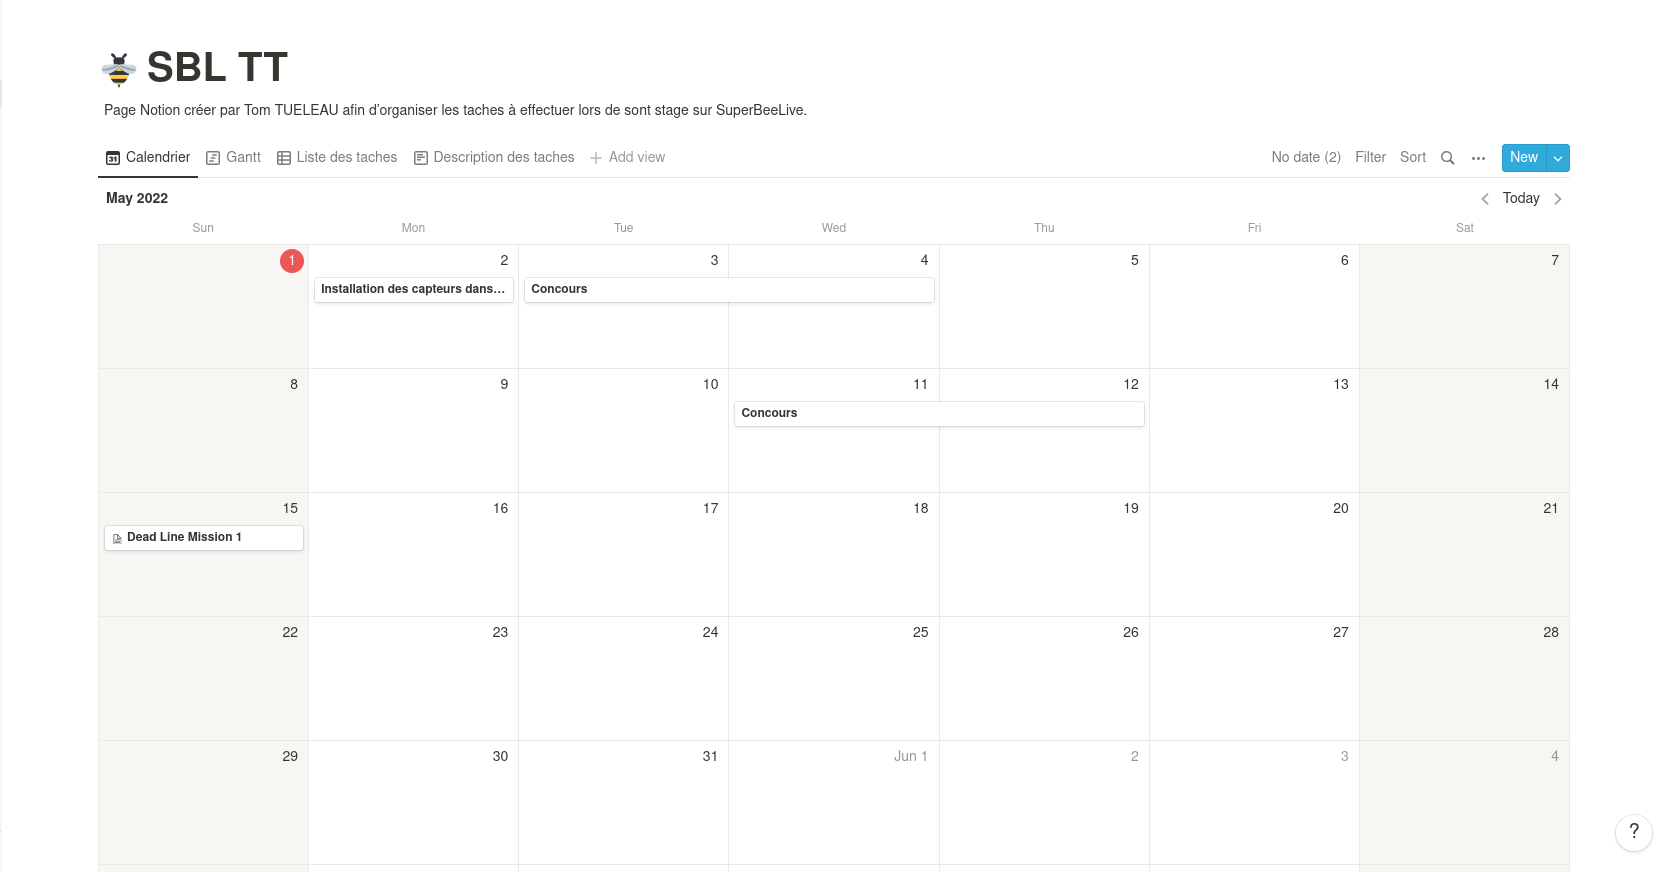
\includegraphics[scale=0.35]{../img/notioncalender.png}
\captionof{figure}{Calendrier}
\label{Calendrier}
\end{center}

\subsubsection{Liste des tâches}
La page liste des tâches regroupe touts les tâches effectuées et à effectuer. J'attribue à ces tâches des étiquettes ce qui me permet de les classer.   
\begin{center}	
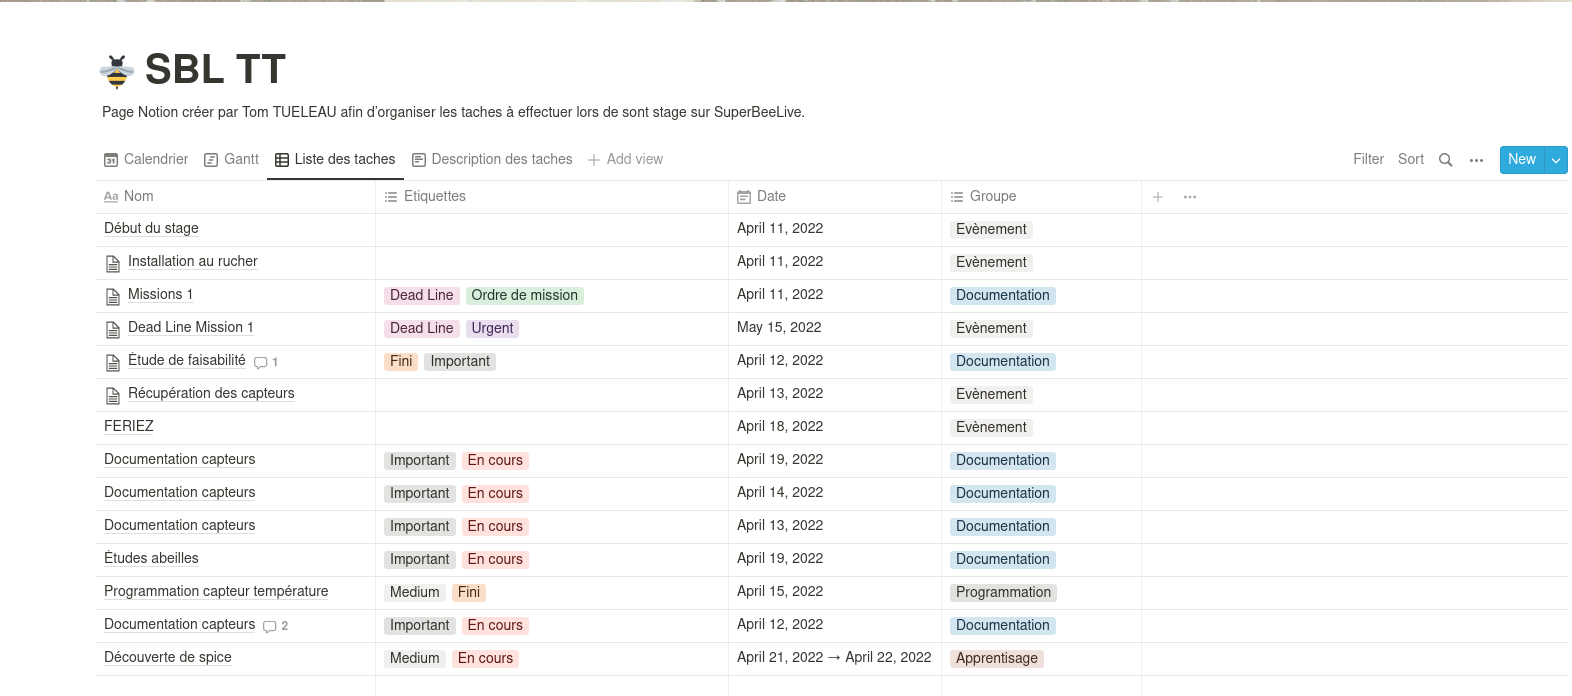
\includegraphics[scale=0.35]{../img/notionlistesdestaches.png}
\captionof{figure}{Liste des taches}
\label{Liste des taches}
\end{center}

\subsubsection{Description des tâches}
Cet onglet contient une description plus détaillée des tâches. J'y stoque aussi les comptes rendus de réunion, prise de note, image relative à mes parties du projet.
\begin{center}	
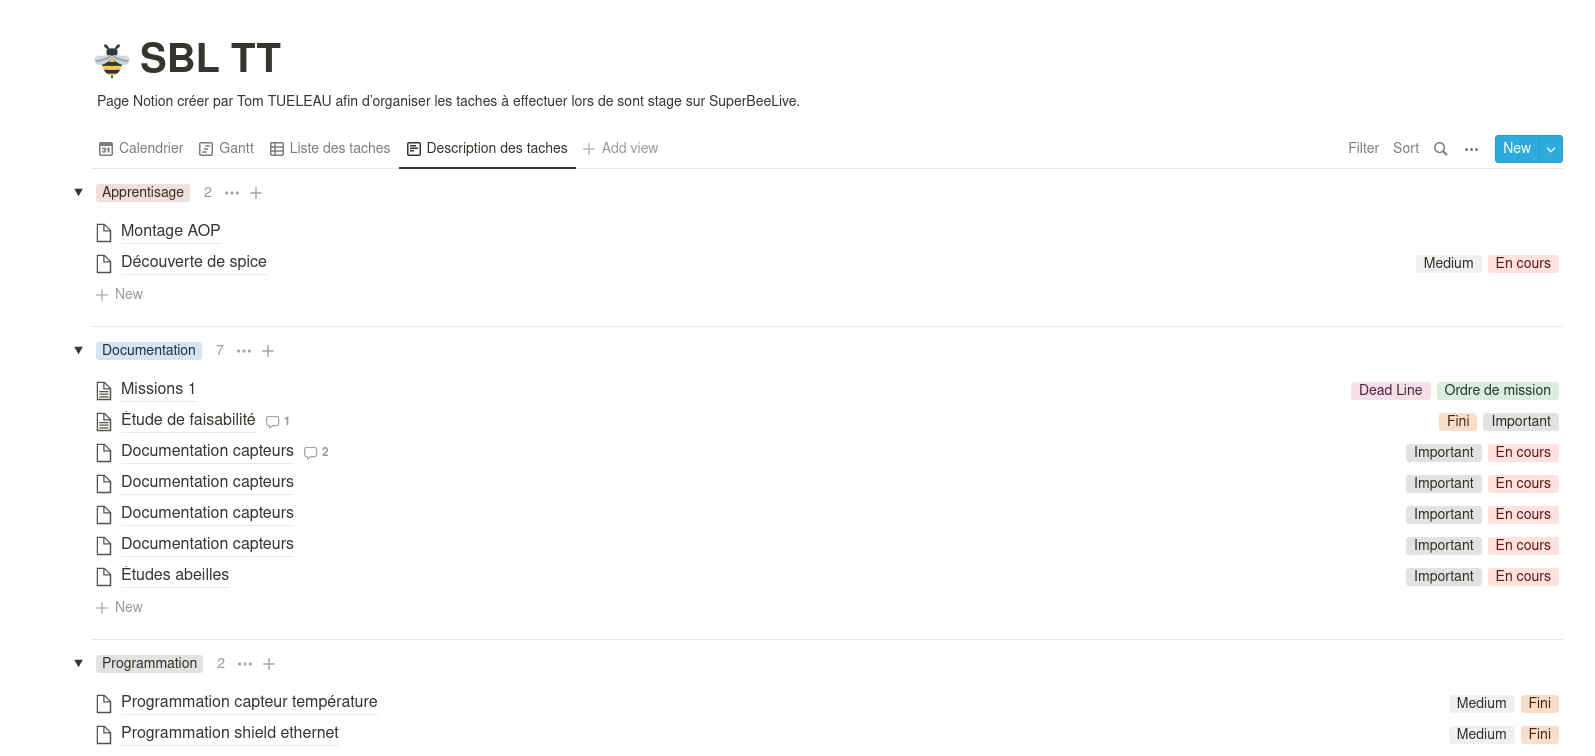
\includegraphics[scale=0.35]{../img/notiondescriptiondestaches.png}
\captionof{figure}{Description des taches}
\label{Description des taches}
\end{center}

\subsubsection{Gantt}
La dernier fiche accessible est la fiche "Gantt" qui me permet surout de m'organiser sur ma semaine. 
\begin{center}	
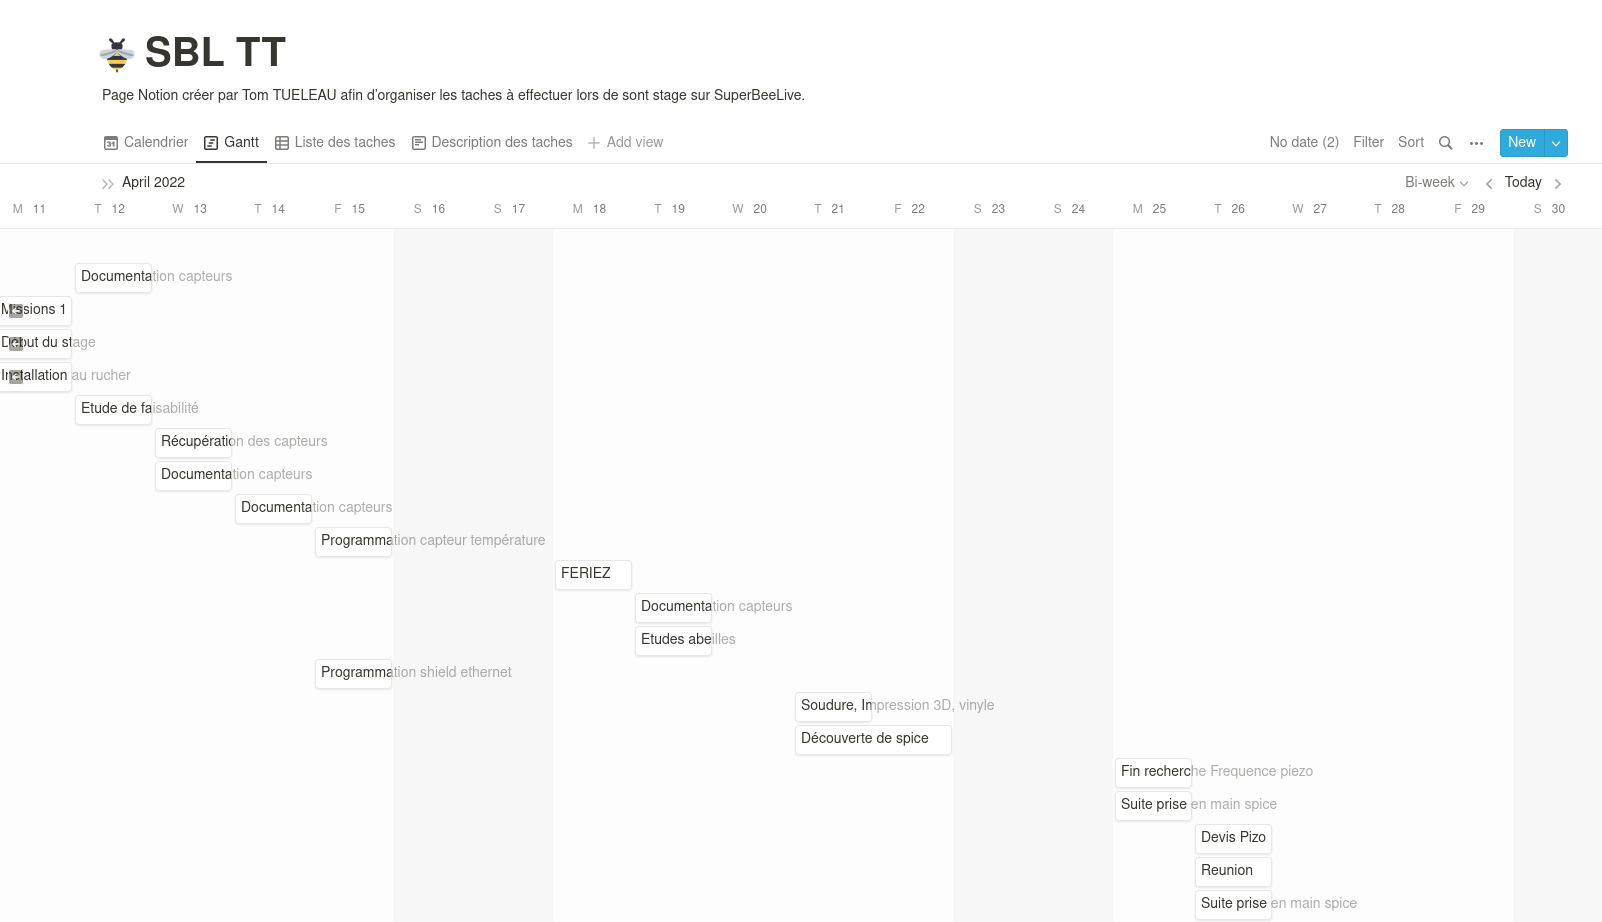
\includegraphics[scale=0.35]{../img/notiongantt.png}
\captionof{figure}{Gantt}
\label{Gantt}
\end{center}
\newpage 
\section{Conclusion}

Les tâches qu'il me reste à effectuer pour les prochaines semaines sont les suivantes :
\\
\\- Mettre en place dans la ruche les capteurs déjà opérationêls
\\- Rendre opérationêl le capteur de vibration en finalisant sur une plaquette de prototypage les montages d'amplification.
\\- Organiser l'affichage des données avec la personne chargée du site Web. 
\\- Reprendre l'analyse du logiciel "Jaaba" de  Kristin Branson. 
\\- Regarder et mettre en fonctionnement le microphone fourni.
\newpage
\listoffigures
\end{document}
